\section{赋权图,最短路径}
\subsection{赋权图}
在图的实际应用中,除了要建立图模型以外,
有时还需要将一些附加信息赋予图的边或顶点,
这就是\emph{赋权图}(weighted graph).
本节仅讨论边赋权图.

\begin{definition}
%@see: 《离散数学》(邓辉文) P186 定义6-33
设\(G = (V,E)\)是简单图,
%TODO 《离散数学》(邓辉文)原书上没有限定“简单”图
%TODO 但是我认为自环和多重边对于赋权图是没有意义的,所以这里自作主张改为简单图
映射\(\omega\colon E \to \mathbb{R}\),
则称“\((G,\omega)\)是\DefineConcept{边赋权图}”,
把\(\omega\)称为“\(G\)的\DefineConcept{边赋权映射}”.
对于任意一条边\(e \in E\),
把\(\omega(e)\)称为“\(e\)的\DefineConcept{权}(weight)”.
\end{definition}

通常我们将映射\(\omega\)的值域限制为非负实数\([0,+\infty)\).

\cref{figure:图论.边赋权有向图1,figure:图论.边赋权无向图1} 就是两个边赋权图.

\begin{figure}[hbt]
%@see: 《离散数学》(邓辉文) P186 图6-39
	\centering
	\def\subwidth{.4\linewidth}
	\begin{subfigure}[b]{\subwidth}
		\centering
		\begin{tikzpicture}
			\fill(0,0)coordinate(v1)node[left]{$v_1$}circle(2pt);
			\fill(1,{sqrt(3)})coordinate(v2)node[above]{$v_2$}circle(2pt);
			\fill(2,0)coordinate(v3)node[right]{$v_3$}circle(2pt);
			\fill(1,{-sqrt(3)})coordinate(v4)node[below]{$v_4$}circle(2pt);
			\fill(3,{-sqrt(3)})coordinate(v5)node[below]{$v_5$}circle(2pt);
			\fill(3,{sqrt(3)})coordinate(v6)node[above]{$v_6$}circle(2pt);
			\fill(4,0)coordinate(v7)node[right]{$v_7$}circle(2pt);
			\begin{scope}[-{Latex[length=3mm,width=0pt 10]}]
				\draw(v1)--(v2)node[midway,left]{2};
				\draw(v1)--(v3)node[midway,above]{5};
				\draw(v1)--(v4)node[midway,left]{3};
				\draw(v2)--(v3)node[midway,right]{2};
				\draw(v2)--(v6)node[midway,above]{7};
				\draw(v3)--(v6)node[midway,right]{5};
				\draw(v3)--(v4)node[midway,left]{1};
				\draw(v3)--(v5)node[midway,left]{3};
				\draw(v4)--(v5)node[midway,below]{5};
				\draw(v5)--(v6)node[midway,right]{1};
				\draw(v5)--(v7)node[midway,right]{7};
				\draw(v6)--(v7)node[midway,right]{5};
			\end{scope}
		\end{tikzpicture}
		\caption{}
		\label{figure:图论.边赋权有向图1}
	\end{subfigure}~\begin{subfigure}[b]{\subwidth}
		\centering
		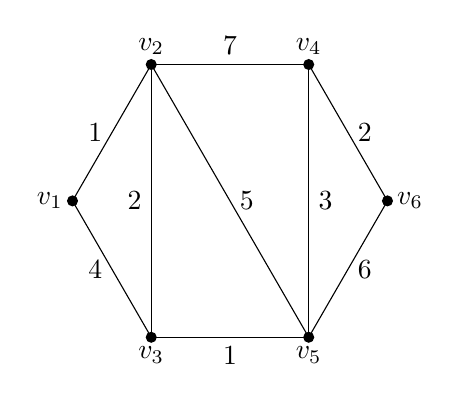
\begin{tikzpicture}
			\fill(0,0)coordinate(v1)node[left]{$v_1$}circle(2pt);
			\fill(1,{sqrt(3)})coordinate(v2)node[above]{$v_2$}circle(2pt);
			\fill(1,{-sqrt(3)})coordinate(v3)node[below]{$v_3$}circle(2pt);
			\fill(3,{sqrt(3)})coordinate(v4)node[above]{$v_4$}circle(2pt);
			\fill(3,{-sqrt(3)})coordinate(v5)node[below]{$v_5$}circle(2pt);
			\fill(4,0)coordinate(v6)node[right]{$v_6$}circle(2pt);
			\draw(v1)--(v2)node[midway,left]{1};
			\draw(v1)--(v3)node[midway,left]{4};
			\draw(v2)--(v3)node[midway,left]{2};
			\draw(v2)--(v4)node[midway,above]{7};
			\draw(v2)--(v5)node[midway,right]{5};
			\draw(v3)--(v5)node[midway,below]{1};
			\draw(v4)--(v5)node[midway,right]{3};
			\draw(v4)--(v6)node[midway,right]{2};
			\draw(v5)--(v6)node[midway,right]{6};
		\end{tikzpicture}
		\caption{}
		\label{figure:图论.边赋权无向图1}
	\end{subfigure}
	\caption{}
\end{figure}

我们可以改进邻接矩阵,用它来表示赋权图.
\begin{itemize}
	\item 如果\(v_i\)与\(v_j\)邻接,具体分为以下两种情况:\begin{itemize}
		\item 当\(G\)是赋权有向图时,
		则\(a_{ij}\)表示以\(v_i\)为起点、\(v_j\)为终点的有向边的权;
		\item 当\(G\)是赋权无向图时,
		\(a_{ij},a_{ji}\)均表示以\(v_i,v_j\)为端点的无向边的权.
	\end{itemize}
	\item 如果\(v_i\)与\(v_j\)不邻接,
	令\(a_{ij} = +\infty\).
\end{itemize}


\subsection{最短路径}
在边赋权图\(G = (V,E)\)中,
从一个顶点到另一个顶点,
路上所有边的权之和,
称为这条路的权.

例如,在\cref{figure:图论.边赋权有向图1} 中,
路\(v_2 v_3 v_5 v_6 v_7\)的权为\(2+3+1+5=11\).

从一个顶点\(v_1\)到另一个顶点\(v_2\)的、权最小的一条路,
称为“从\(v_1\)到\(v_2\)的\DefineConcept{最短路径}”.
